\documentclass{standalone}
\usepackage{tikz}
\usetikzlibrary{patterns, positioning}
\usepackage[sfdefault]{ClearSans} %% option 'sfdefault' activates Clear Sans as the default text font
\usepackage[T1]{fontenc}

\begin{document}
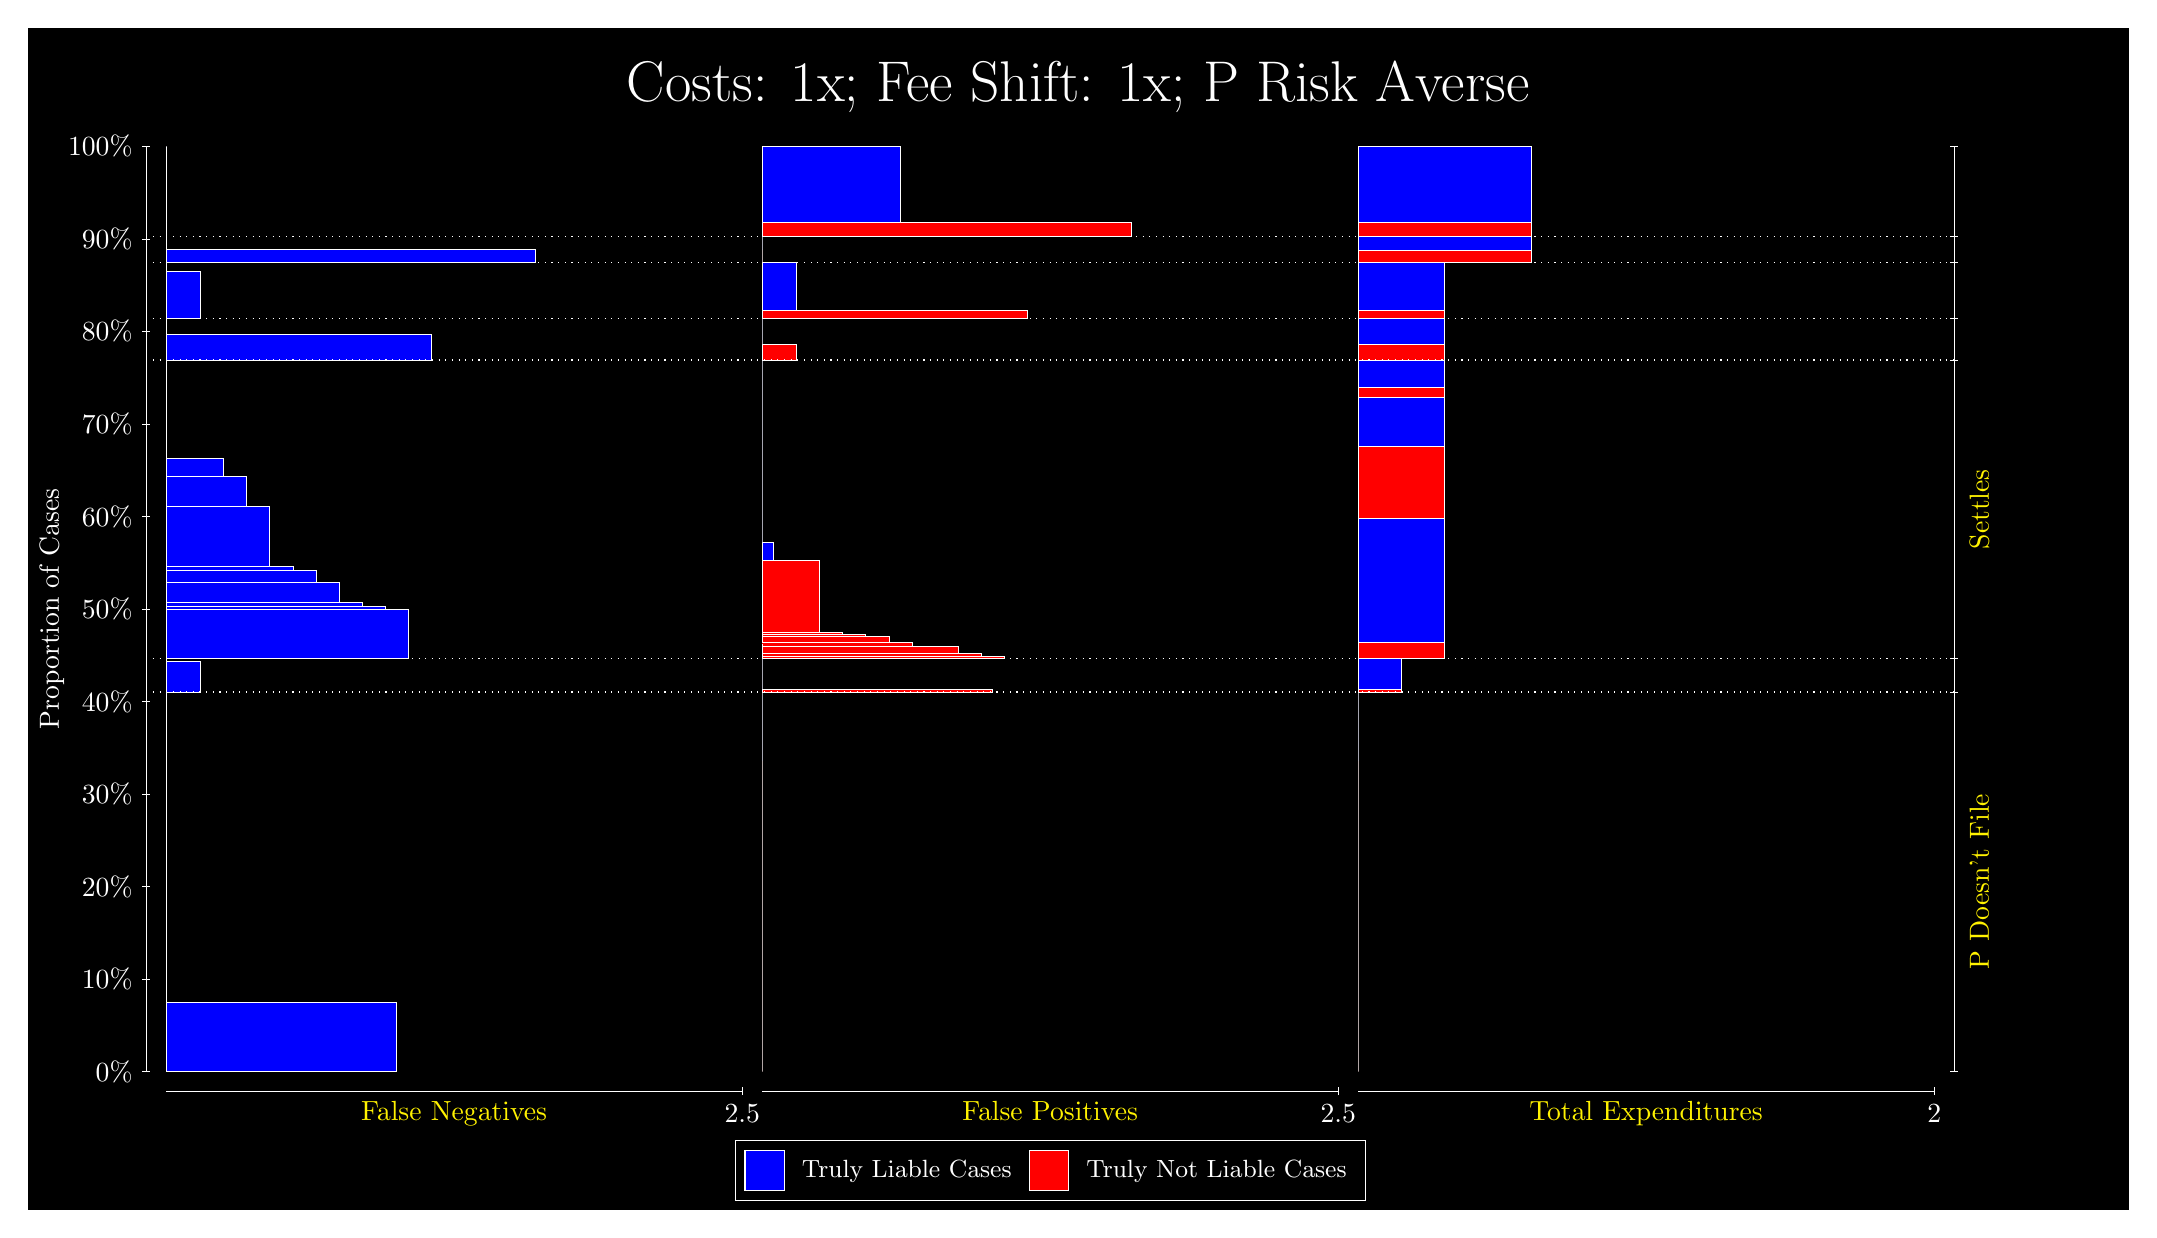
\begin{tikzpicture}
\draw[fill=black] (0,0) rectangle (26.667,15);
\draw[text=white] (0,13.5) rectangle (26.667,15) node[midway] {\huge Costs: 1x; Fee Shift: 1x; P Risk Averse};
\draw[white, very thin] (1.5,1.75) -- (1.5,13.5);
\node[rotate=90, text=white, anchor=center] at (0.3, 7.625) {Proportion of Cases};
\draw[white, very thin] (1.45,1.75) -- (1.55,1.75);
\node[text=white, anchor=east] at (1.45, 1.75) {0\%};
\draw[white, very thin] (1.45,2.925) -- (1.55,2.925);
\node[text=white, anchor=east] at (1.45, 2.925) {10\%};
\draw[white, very thin] (1.45,4.1) -- (1.55,4.1);
\node[text=white, anchor=east] at (1.45, 4.1) {20\%};
\draw[white, very thin] (1.45,5.275) -- (1.55,5.275);
\node[text=white, anchor=east] at (1.45, 5.275) {30\%};
\draw[white, very thin] (1.45,6.45) -- (1.55,6.45);
\node[text=white, anchor=east] at (1.45, 6.45) {40\%};
\draw[white, very thin] (1.45,7.625) -- (1.55,7.625);
\node[text=white, anchor=east] at (1.45, 7.625) {50\%};
\draw[white, very thin] (1.45,8.8) -- (1.55,8.8);
\node[text=white, anchor=east] at (1.45, 8.8) {60\%};
\draw[white, very thin] (1.45,9.975) -- (1.55,9.975);
\node[text=white, anchor=east] at (1.45, 9.975) {70\%};
\draw[white, very thin] (1.45,11.15) -- (1.55,11.15);
\node[text=white, anchor=east] at (1.45, 11.15) {80\%};
\draw[white, very thin] (1.45,12.325) -- (1.55,12.325);
\node[text=white, anchor=east] at (1.45, 12.325) {90\%};
\draw[white, very thin] (1.45,13.5) -- (1.55,13.5);
\node[text=white, anchor=east] at (1.45, 13.5) {100\%};

\draw[white, very thin] (24.457,1.75) -- (24.457,13.5);
\draw[white, very thin] (24.407,1.75) -- (24.507,1.75);
\node[anchor=west] at (24.407, 1.75) {};
\draw[white, very thin] (24.407,6.5704) -- (24.507,6.5704);
\node[anchor=west] at (24.407, 6.5704) {};
\draw[white, very thin] (24.407,6.9952) -- (24.507,6.9952);
\node[anchor=west] at (24.407, 6.9952) {};
\draw[white, very thin] (24.407,10.787) -- (24.507,10.787);
\node[anchor=west] at (24.407, 10.787) {};
\draw[white, very thin] (24.407,11.314) -- (24.507,11.314);
\node[anchor=west] at (24.407, 11.314) {};
\draw[white, very thin] (24.407,12.022) -- (24.507,12.022);
\node[anchor=west] at (24.407, 12.022) {};
\draw[white, very thin] (24.407,12.358) -- (24.507,12.358);
\node[anchor=west] at (24.407, 12.358) {};
\draw[white, very thin] (24.407,13.5) -- (24.507,13.5);
\node[anchor=west] at (24.407, 13.5) {};

\draw[white, very thin, fill=blue] (1.75,1.75) rectangle (4.6775,2.6251);
\draw[white, very thin, fill=red] (1.75,2.6251) rectangle (1.75,6.5704);
\draw[white, very thin, fill=blue] (1.75,6.5704) rectangle (2.1891,6.9557);
\draw[white, very thin, fill=red] (1.75,6.9557) rectangle (1.75,6.9952);
\draw[white, very thin, fill=blue] (1.75,6.9952) rectangle (4.8239,7.6185);
\draw[white, very thin, fill=blue] (1.75,7.6185) rectangle (4.5312,7.6603);
\draw[white, very thin, fill=blue] (1.75,7.6603) rectangle (4.2384,7.7076);
\draw[white, very thin, fill=blue] (1.75,7.7076) rectangle (3.9457,7.965);
\draw[white, very thin, fill=blue] (1.75,7.965) rectangle (3.6529,8.1203);
\draw[white, very thin, fill=blue] (1.75,8.1203) rectangle (3.3602,8.163);
\draw[white, very thin, fill=blue] (1.75,8.163) rectangle (3.0674,8.9232);
\draw[white, very thin, fill=blue] (1.75,8.9232) rectangle (2.7746,9.3159);
\draw[white, very thin, fill=blue] (1.75,9.3159) rectangle (2.4819,9.5417);
\draw[white, very thin, fill=red] (1.75,9.5417) rectangle (1.75,10.787);
\draw[white, very thin, fill=blue] (1.75,10.787) rectangle (5.1167,11.116);
\draw[white, very thin, fill=red] (1.75,11.116) rectangle (1.75,11.314);
\draw[white, very thin, fill=blue] (1.75,11.314) rectangle (2.1891,11.914);
\draw[white, very thin, fill=red] (1.75,11.914) rectangle (1.75,12.022);
\draw[white, very thin, fill=blue] (1.75,12.022) rectangle (6.4341,12.197);
\draw[white, very thin, fill=red] (1.75,12.197) rectangle (1.75,12.358);
\draw[white, very thin, fill=red] (1.75,12.358) rectangle (1.75,12.536);
\draw[white, very thin, fill=blue] (1.75,12.536) rectangle (1.75,13.5);
\draw[white, very thin, fill=red] (9.3189,1.75) rectangle (9.3189,5.6953);
\draw[white, very thin, fill=blue] (9.3189,5.6953) rectangle (9.3189,6.5704);
\draw[white, very thin, fill=red] (9.3189,6.5704) rectangle (12.246,6.6099);
\draw[white, very thin, fill=blue] (9.3189,6.6099) rectangle (9.3189,6.9952);
\draw[white, very thin, fill=red] (9.3189,6.9952) rectangle (12.393,7.0182);
\draw[white, very thin, fill=red] (9.3189,7.0182) rectangle (12.1,7.0594);
\draw[white, very thin, fill=red] (9.3189,7.0594) rectangle (11.807,7.1474);
\draw[white, very thin, fill=red] (9.3189,7.1474) rectangle (11.515,7.1542);
\draw[white, very thin, fill=red] (9.3189,7.1542) rectangle (11.222,7.1963);
\draw[white, very thin, fill=red] (9.3189,7.1963) rectangle (10.929,7.1972);
\draw[white, very thin, fill=red] (9.3189,7.1972) rectangle (10.929,7.2799);
\draw[white, very thin, fill=red] (9.3189,7.2799) rectangle (10.636,7.3026);
\draw[white, very thin, fill=red] (9.3189,7.3026) rectangle (10.344,7.3236);
\draw[white, very thin, fill=red] (9.3189,7.3236) rectangle (10.051,8.2406);
\draw[white, very thin, fill=blue] (9.3189,8.2406) rectangle (9.4652,8.4664);
\draw[white, very thin, fill=blue] (9.3189,8.4664) rectangle (9.3189,10.787);
\draw[white, very thin, fill=red] (9.3189,10.787) rectangle (9.758,10.984);
\draw[white, very thin, fill=blue] (9.3189,10.984) rectangle (9.3189,11.314);
\draw[white, very thin, fill=red] (9.3189,11.314) rectangle (12.686,11.421);
\draw[white, very thin, fill=blue] (9.3189,11.421) rectangle (9.758,12.022);
\draw[white, very thin, fill=red] (9.3189,12.022) rectangle (9.3189,12.184);
\draw[white, very thin, fill=blue] (9.3189,12.184) rectangle (9.3189,12.358);
\draw[white, very thin, fill=red] (9.3189,12.358) rectangle (14.003,12.536);
\draw[white, very thin, fill=blue] (9.3189,12.536) rectangle (11.075,13.5);
\draw[white, very thin, fill=red] (16.888,1.75) rectangle (16.888,5.6953);
\draw[white, very thin, fill=blue] (16.888,5.6953) rectangle (16.888,6.5704);
\draw[white, very thin, fill=red] (16.888,6.5704) rectangle (17.437,6.6099);
\draw[white, very thin, fill=blue] (16.888,6.6099) rectangle (17.437,6.9952);
\draw[white, very thin, fill=red] (16.888,6.9952) rectangle (17.986,7.1972);
\draw[white, very thin, fill=blue] (16.888,7.1972) rectangle (17.986,8.7777);
\draw[white, very thin, fill=red] (16.888,8.7777) rectangle (17.986,9.6947);
\draw[white, very thin, fill=blue] (16.888,9.6947) rectangle (17.986,10.318);
\draw[white, very thin, fill=red] (16.888,10.318) rectangle (17.986,10.444);
\draw[white, very thin, fill=blue] (16.888,10.444) rectangle (17.986,10.787);
\draw[white, very thin, fill=red] (16.888,10.787) rectangle (17.986,10.984);
\draw[white, very thin, fill=blue] (16.888,10.984) rectangle (17.986,11.314);
\draw[white, very thin, fill=red] (16.888,11.314) rectangle (17.986,11.421);
\draw[white, very thin, fill=blue] (16.888,11.421) rectangle (17.986,12.022);
\draw[white, very thin, fill=red] (16.888,12.022) rectangle (19.083,12.184);
\draw[white, very thin, fill=blue] (16.888,12.184) rectangle (19.083,12.358);
\draw[white, very thin, fill=red] (16.888,12.358) rectangle (19.083,12.536);
\draw[white, very thin, fill=blue] (16.888,12.536) rectangle (19.083,13.5);
\draw[white, dotted] (1.5,6.5704) -- (24.457,6.5704);
\draw[white, dotted] (1.5,6.9952) -- (24.457,6.9952);
\draw[white, dotted] (1.5,10.787) -- (24.457,10.787);
\draw[white, dotted] (1.5,11.314) -- (24.457,11.314);
\draw[white, dotted] (1.5,12.022) -- (24.457,12.022);
\draw[white, dotted] (1.5,12.358) -- (24.457,12.358);
\draw[white, very thin] (1.75,1.5) -- (9.0689,1.5);
\node[text=yellow, anchor=north] at (5.4094, 1.5) {False Negatives};
\draw[white, very thin] (9.0689,1.45) -- (9.0689,1.55);
\node[text=white, anchor=north] at (9.0689, 1.45) {2.5};

\draw[white, very thin] (9.3189,1.5) -- (16.638,1.5);
\node[text=yellow, anchor=north] at (12.978, 1.5) {False Positives};
\draw[white, very thin] (16.638,1.45) -- (16.638,1.55);
\node[text=white, anchor=north] at (16.638, 1.45) {2.5};

\draw[white, very thin] (16.888,1.5) -- (24.207,1.5);
\node[text=yellow, anchor=north] at (20.547, 1.5) {Total Expenditures};
\draw[white, very thin] (24.207,1.45) -- (24.207,1.55);
\node[text=white, anchor=north] at (24.207, 1.45) {2};

\node[text=yellow, centered, rotate=90] at (24.777, 4.1602) {P Doesn't File};

\node[text=yellow, centered, rotate=90] at (24.777, 8.8912) {Settles};





\draw (12.978300999999998,1.5) node[draw=none] (baseCoordinate) {};
\begin{scope}[align=center]
        \matrix[scale=0.5, draw=white, below=0.5cm of baseCoordinate, nodes={draw}, column sep=0.1cm]{
            \node[rectangle, draw, minimum width=0.5cm, minimum height=0.5cm, fill=blue] {}; &
            \node[draw=none, font=\small, text=white] (B) {Truly Liable Cases}; &
            \node[rectangle, draw, minimum width=0.5cm, minimum height=0.5cm, fill=red] {}; &
            \node[draw=none, font=\small, text=white] (B) {Truly Not Liable Cases}; \\
            };
\end{scope}

\end{tikzpicture}
\end{document}